In this chapter the results of our research project will be presented. First, will be diven into the architecture of web browsers. This will mostly be about the different process models and network stacks of the populair browsers. This was a prerequisite for the design and development of our algorithm that will be described in the second part of this chapter. In the last part of this chapter will be focussed on the results of the implemention and usage of the algorithm to detect real malware \todo{Better description} in a fast and reliable way.
Although, support for this was added pretty quickly using tabs, this left us with a problem to detect when a new URL was feeded to a tab\todo{See problems below}. To solve this problem, every URL is now opened in its own window.
\begin{description}
\item[on\_process\_new] sfdsfdf
\item[on\_process\_finished] sfdsfdf
\item[on\_http\_request] sfdsfdf
\item[on\_file\_write] sfdsfdf
\item[on\_file\_delete] sfdsfdf
\item[on\_registry\_set] sfdsfdf
\item[on\_registry\_delete] sfdsfdf
\item[on\_shell\_execute] sfdsfdf
\item[on\_socket\_connect] sfdsfdf
\item[on\_anomaly\_detected] sfdsfdf
\end{description}
\subsubsection{Analyzer}

To implement the analysis phase of the algorithm, a simple analyzer was written that detects process spawns below browsing contexts.

\begin{lstlisting}
function deep_process_spawn_analyzer(graph)
    foreach vertex in graph
        if vertex.type == "process_spawned"
            if check_depth_in_graph(vertex, 0) > 1
                print "Malicious activity"
            endif
        endif
    endforeach
endfunction

function check_depth_in_graph(vertex, current_depth)
    parents = get_parents_of_vertex(vertex)
    # Actually we need only one parent
    if length_array(parents) > 0
        return check_depth_in_graph(parents[0], current_depth++)
    else
        # No more parents, we're at the root node
        return current_depth
    endif
endfunction
\end{lstlisting}
\todo{Betere analyzer reporting in output script...}
\begin{lstlisting}
$ python cuckoo.py &
$ python utils/mass-analyse.py -g -t 22
Warning: Task with ID 22 is not yet completed; Waiting...
INFO:root:Parse log....
Analyzer 'Subprocess_from_tab': The URL 'http://malware-site.com' 
spawns a process called 'errfix.exe'.
\end{lstlisting}

\newgeometry{left=3cm,top=0.1cm,bottom=0.1cm}
 \todo{Explain the colors of the vertices}
\begin{figure}[h]
    \centering
    \includegraphics[width=17cm]{Images/graph2.png}
    \caption{An example of the graph}
    \label{fig:graph}
\end{figure}
\subsubsection{Step 6}
\begin{figure}[h]
    \centering
    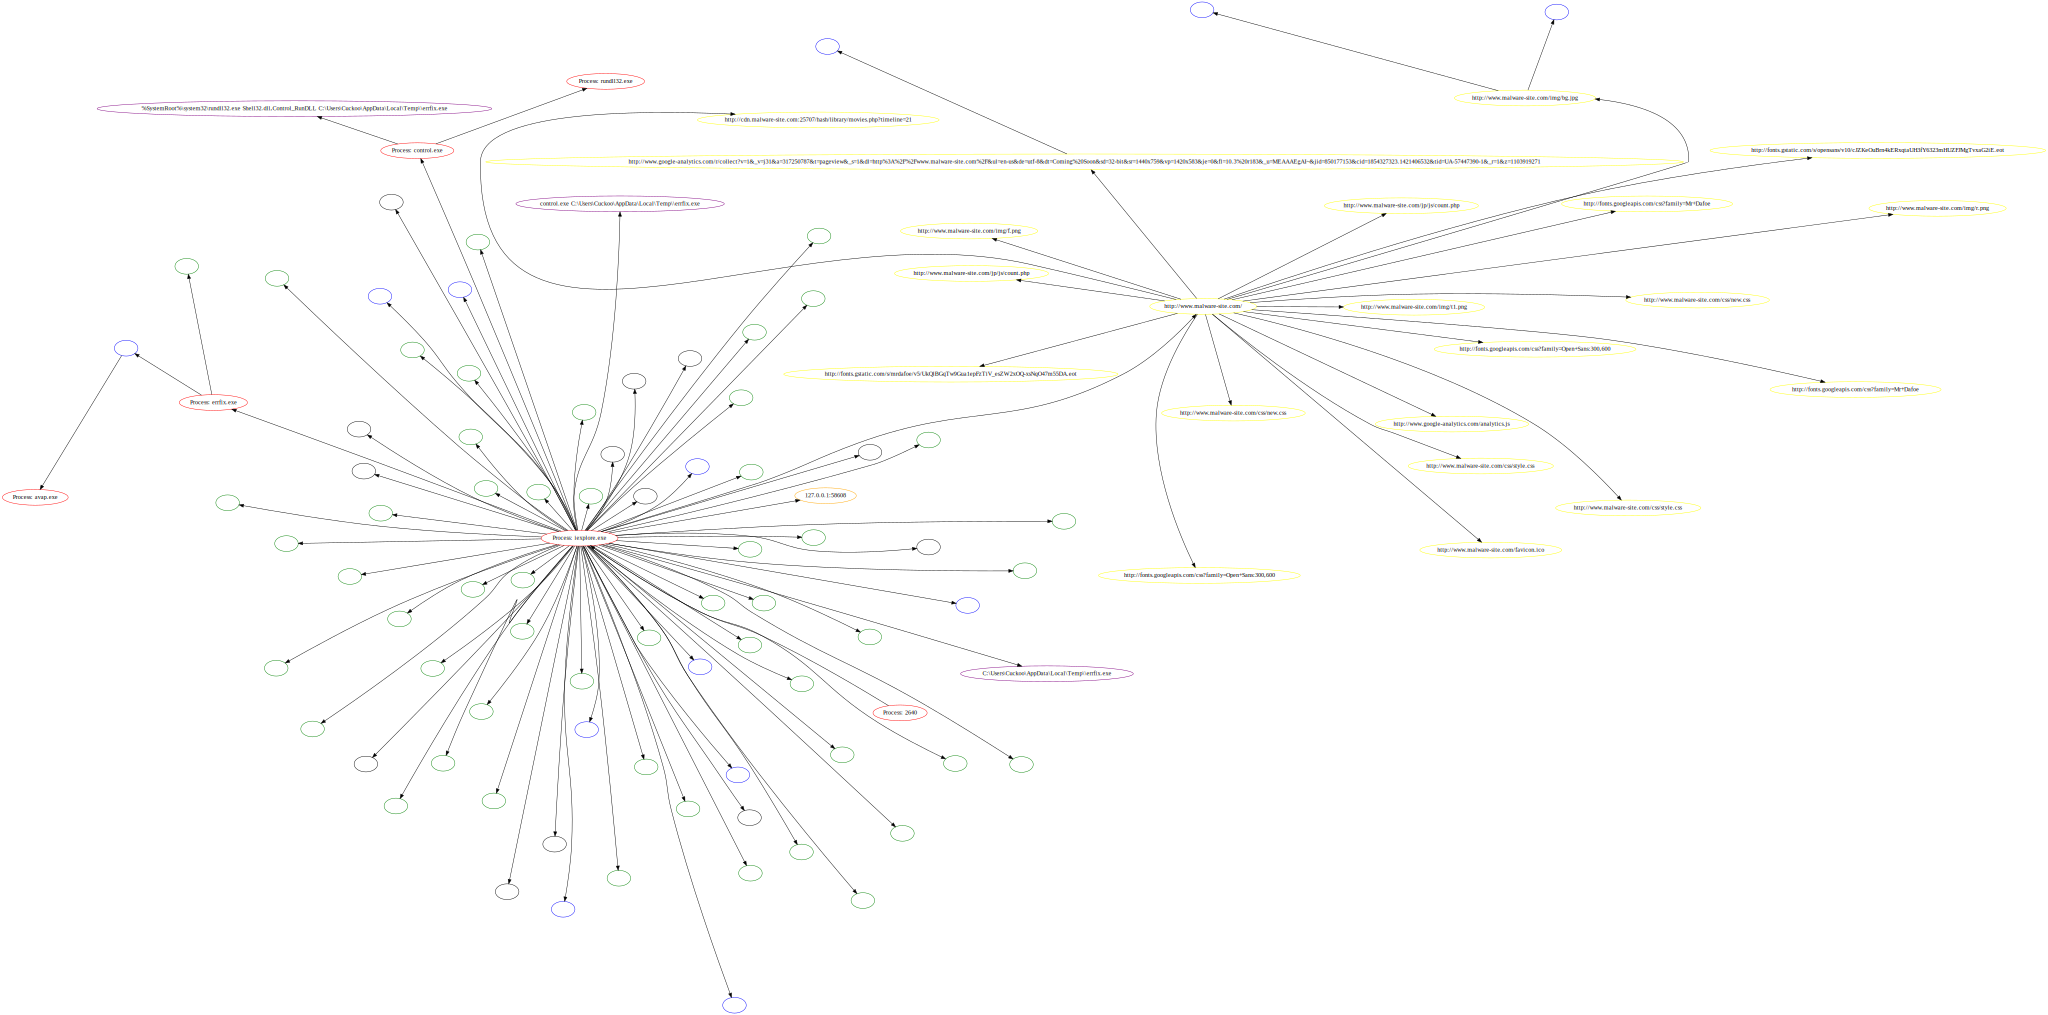
\includegraphics[width=25cm, angle=90]{Images/report_Subprocess_from_tab}
    \caption{An example of the subgraph of a single website that injected the virtual machine with malware. For clarity are only the labels of the nodes of visited URLs, involved processes and executed shell commands showed.}
    \label{fig:subgraph}
\end{figure}

\restoregeometry
\subsubsection{Improvements}

\todo{Speedboost tussen Cuckoo 1.2-dev en onze wijzigingen in grafiekje zetten}



\subsubsection{Problems}
\label{99problems}
\epigraph{I've got 99 problems but Cuckoo ain't one.}{Adriaan}

\begin{itemize}
\item Out of order openen en sluiten van handles 
\item Paralellizatie problemen
\item BSON file loggen naar de host
\item Weten wanneer een nieuwe URL wordt geopend
\begin{itemize}
\item Geen TypedURLs met COM
\item COM (CrossZoneCompare, blocking Navigate met deadlock tot gevolg, )
\end{itemize}
\item Opsplitsen / linken van de data in 1 process over meerdere requests
\item Missende data door te kleine buffers en niet geimplementeerde apis in cuckoomon
\end{itemize}
